\documentclass[11pt]{article}
\usepackage{cite}
\usepackage{fancyhdr}
\usepackage[svgnames]{xcolor}
\usepackage{url}
\usepackage{tikz}
\usetikzlibrary{shapes,snakes,arrows}
\usepackage{hyperref}

\topmargin=-5mm
\evensidemargin=0cm
\oddsidemargin=0cm
\textwidth=16cm
\textheight=22cm
\addtolength{\headheight}{1.6pt}
\hypersetup{pdfstartview=}

\tikzset{>=latex}

\newcommand{\lastupdate}{\today}
\newcommand{\ie}{\textit{i.e.}}
\newcommand{\mdash}{---}
\newcommand{\ecall}{\textsf{ecall}}
\newcommand{\ocall}{\textsf{ocall}}
\newcommand{\env}{\textsf{environment}}
\newcommand{\mrenclave}{\textsf{mrenclave}}
\newcommand{\mrsigner}{\textsf{mrsigner}}
\newcommand{\sha}{\textsf{sha256}}

% \lhead{\sc On the insufficiency of Intel SGX Remote Attestation}
% \rhead{\sc \lastupdate}

\title{\bf A Framework for analyzing Intel SGX Enclaves}
\author{\textsc{Yogesh Prem Swami}}

\date{\lastupdate}

\begin{document}
\pagenumbering{arabic}

\maketitle

\begin{abstract}
  Intel SGX enclaves  provide hardware
  enforced confidentiality and integrity guarantees for running pure
  computations (\ie, OS-level side-effect-free code) in the cloud
  environment. In addition, SGX remote attestation enables
  enclaves to prove that a claimed enclave is indeed running inside a
  genuine SGX hardware and not some (adversary controlled) SGX
  simulator.

  Since cryptographic protocols do not compose well
  \cite{ucframework} especially when run concurrently, SGX remote
  attestation is only a necessary pre-condition for securely
  instantiating an enclave. In practice, one needs to analyze all the
  different interacting enclaves as a single protocol and make sure
  that no sub-computation of the protocol can be simulated outside of
  the enclave. In this paper, we present a practical framework for
  analyzing enclaves. We analyze Intel provided EPID\cite{epid}
  \textsf{Provisioning} and \textsf{Quoting} Enclave\cite{sgxattest}
  within this framework and report our (largely positive) findings. We
  also provide details about SGX's use of EPID and report
  (largely negative) results about claimed anonymity guarantees.
\end{abstract}

\section{Introduction}
  Intel SGX enclaves\cite{sgxinnov, sgxinnov2} provide hardware
  enforced confidentiality and  integrity guarantees for running pure
  computation (\textit{i.e.}, OS-level side-effect-free code) in the
  cloud environment. By limiting the application's Trusted Computing
  Base (TCB) to the CPU and CPU-Cache, SGX provides unprecidented
  confidentiality and integrity guarantees against malicious OS
  kernels and supervisor software. Since a remote user cannot be sure
  if an enclave is indeed running on a real-hardware instead of a
  software simulator (such as QEMU), SGX provides a remote attestation
  mechanism to prove to third parties that an enclave has indeed been
  instantiated on a real hardware.

  Given such strong guarantees, a popular design methodology for
  creating secure cloud applications is to:

  \begin{itemize}
    \item Compose multiple independent well-known protocols inside the
      enclave to create a larger protocol, and

    \item Depend on remote attestation to ensure that different parts
      of the protocol can only
  \end{itemize}

  Good examples of this methodology are \cite{Haven, Graphene, Scone},
  where the authors try to run unmodified (or minimally modified)
  applications inside the enclave, and depend upon remote-attestation
  to make sure that the internal state of the application will not be
  compromise.


  \section{SGX Computational Model}
  Intel documentation\cite{intelsdm} provides excellent low-level
  details about the SGX instructions. This section provides an
  abstract computational model of SGX which is better suited for
  security analysis of an SGX enclave.

  Abstractly, an SGX enclave can be thought of as a blackbox that's
  capable of running any arbitrary algorthim. The blackbox, hereafter
  called an enclave, communicates with the outside world, called the
  \env, in three different ways:

  \begin{description}
  \item[Ecall]: The \env\ can invoke a pre-defined function inside the
    enclave by passing input parameters and returning internal state
    of the enclave as results. Such invocations from the \env\ to the
    enclave are referred to as \ecall. The parameter values passed
    from the \env\ to the enclave are either coped or directly shared
    with the enclave. An \ecall\ can terminate in one of the three
    ways: (a) by returning from the enclave, (b) by making an explicit
    \ocall, or (c) as a result of an interrupt or exception.

    SGX also supports multithreading, and it's possible for the
    \env\ to run the same \ecall\ in different threads. However, once
    an \ecall\ has acquired the thread, future attempts to reuse that
    same thread will result in error. Futhermore, the number of
    threads that an enclave can support is pre-determined by the
    enclave signer, and cannot be altered at runtime.

  \item [Ocall]: While an enclave is executing (because of some
    previous \ecall), it can make \ocall s  to pre-designated
    functions in the \env.  Unlike an \ecall, an \ocall\ cannot
    directly share the internal enclave state with the \env, and
    must---directly or indirectly---copy the parameters into the
    \env\ before making an \ocall.

    An interesting characteristic of an \ocall\ is that the \env\ is
    not requred to return back to the enclave at the end of the
    \ocall. Since the behavior of pre-designated functions in the
    \env\ are controlled by the adversary, one should not expect the
    \env\ to follow the protocol that enclave author envisioned. In
    particular, it's possible to create a chain of \ecall s and \ocall
    s such that the adversary can perform operations on the internal
    (global) state of the enclave.

  \item[Asynchrnonous Exit] In addition to an \ocall, the
    processor can exit from an enclave due to an interrupt or
    exception. Such enclave exiting events are called Asynchronous
    Exit Events, or AEX. Unlike an \ocall, an AEX can transfer control
    from the enlave to the environment at arbitrary (possibly adversary
    controlled) points inside the enclave. Like \ocall s, an AEX can
    either by resumed from where the enclave left off, or the
    environment can invoke another \ecall (either within the same
    thread or a different thread).
  \end{description}

  \begin{center}
  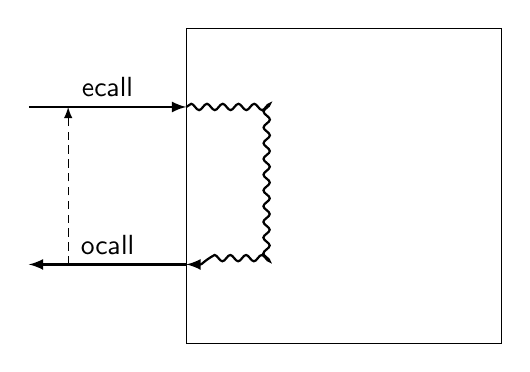
\begin{tikzpicture}[x=1cm, y=-1cm]
  \newcommand{\ench}{4cm}
  \newcommand{\encw}{4cm}
  \newcommand{\alen}{1cm}
  \newcommand{\adiff}{1cm}

  \node[rectangle, minimum height=\ench, minimum width=\encw, draw] (enc) {};
  \draw[->,thick] (-\encw / 2.0 - 2*\alen, \adiff ) -- (-\encw/2.0, \adiff) %%
  node [midway, above] {\textsf{ecall}};

  \draw [->, thick, decorate, %%
    decoration={snake,amplitude=.4mm,segment length=2mm, post length=1mm}] %%
  (-\encw/2.0, \adiff) -- (-\encw/2.0 + 1*\adiff + 0.1, \adiff) -- %%
  (-\encw/2.0 + 1*\adiff , -\adiff) -- (-\encw/2.0, -\adiff);


  \draw[<-,thick] (-\encw / 2.0 - 2*\alen, -\adiff ) -- (-\encw/2.0, -\adiff) %%
  node [midway, above] {\textsf{ocall}};

  \draw[->, thin,densely dashed] (-\encw / 2.0 - 1.5*\alen, -\adiff ) -- %%
  (-\encw/2.0 - 1.5*\alen , \adiff);
\end{tikzpicture}

  \end{center}

  \subsection{Enclave Creation}
  An enclave is generated as a dynamically shared library using
  standard compiler tools. In addition, the entity creating the
  enclave must also decide up front on the following information:  (a)
  stack size of the enclave, (b) heap size of the enclave, (c) number
  of possible threads that can run concurrently, and (d) any other
  auxilary information such as software version, etc.

  Once all these parameters are finalized, the virtual layout of the
  enclave is created in memory and \sha,  hash of then
  entire memory layout (including the stack, heap, thread control
  structure, etc.) are computed (See \cite{intelsdm} for details
  about how the hash is computed). This hash, called
  \mrenclave, is used as the unique identity of the enclave.

  In addition to \textsf{mrenclave}, the software vendor must
  also sign the enclave using a RSA-3072 key. The hash of the RSA
  Public-Key is called \mrsigner. As described in
  \cite{surnaming}, the purpose of the signature is to provide an
  unforgeable identity---a \textit{surname} based lineage---to a set
  of enclaves based on the vendor.

  It should be noted that the \mrenclave\ of an enclave doesn't
  change even when the signing key is changed. This is
  significant when validating attestation or deriving keys based on
  \mrenclave.

  \subsection{Enclave Instantiation and Access Control}
  An properly signed enclave can run on any Intel SGX Processor. SGX
  provides minimal access control through the use of launch enclave
  and enclave white-listing.

  \subsection{SGX Platform Keys}
  \subsection{SGX Platform Enclaves}

  \section{Framework for Analyzing SGX Enclave}
  \subsection{Concurrent Enclave Execution}
  \subsection{Parallel Enclave Execution}
  \subsection{Enclave Rewinding}

  \section{SGX Remote Attestation}
  \subsection{EPID Overview}
  \subsection{SGX Pairing Groups}
  \subsection{SGX EPID provisioning}
  \subsection{SGX Quoting Enclave}

  \section{Alternatives to Remote Attestation}
  \section{Conclusion}

\bibliographystyle{alpha}
\bibliography{sgx_biblio}

\end{document}
